\chapter{考察}
\label{chap:discussion}

本章では,Gyaonについての考察を行う。

\newpage

\section{単純な録音操作による音声活用の促進}
一般的な録音システムでは録音開始/停止それぞれにボタン操作が必要であり、
外部で音声を利用する場合はPC等に音声ファイルをエクスポートしなければならない。
Gyaonでは録音ボタンを押している間録音し、停止後直ちに音声のアップロードが開始される手順となっており、単純な録音操作を実現している。

\subsection{録音コストの軽減}

著者は開発時から継続的にGyaonを使用しており、単純な録音操作によって、録音行為に対する心理的障壁が低くなったと感じている。
このことから、以前まで手書きやキーボード入力していたメモなどを全て録音するようになり、音声を活用する場面が増えた。

\subsection{研究会での活用}
著者の所属する増井研究会でも、Gyaonによって音声活用が促進された。

様々な素材の叩打音を分析する研究が行われており、そこではサンプリングのためにGyaonが活用された。
音声をすぐに確認でき、コメントを付けられる点が好評であった。

また大学が主催する研究発表イベントではリアルタイムな情報共有に活用された。
ブース展示がメインのイベントであったため、面白い展示を見つけた学生がGyaonで共有したり、
楽器のブースでは演奏を録音するなどした。
増井研究会のブースでは常にGyaonを起動していたので、有益な情報を見逃すことなく受け取ることができた。

%共有しやすい
%   URLがあるので「これ聞け」がすぐできる
%
%長時間の音声を録るのはむずい
%   ボタンを押し続けるのは疲れる

%PCもスマホも手元にない時はどうしようもない
%   録音機をばら撒くと解決するかも
%今までのテキストメモに加えて音声メモも管理しないといけない
%   1か所に情報を溜めたいという欲求がある

\subsection{雰囲気記録システムとしての活用}
スマートフォンでも簡単に録音できることから、その場の雰囲気を記録する用途に活用された。
鳥のさえずりや川のせせらぎといった環境音を記録して自宅で聞いたり、研究会のミーティングを録音し、
それを振り返りながらメンバーと懐かしむような場面もあった。

\subsection{楽器練習支援システムとしての活用}
Gyaonペダルとプレビュー再生機能の組み合わせによって、楽器練習支援システムとして便利に活用できた。
楽器演奏において自分の演奏を客観的に評価することは難しいが、録音を行うことによって解決される。
Gyaonペダルを利用すれば演奏中でも録音でき、録音後のプレビュー再生で演奏をすぐに確認することができる。
演奏/録音/確認を素早く行えることから、従来の録音機では実現できなかった新しい練習形態を生み出したといえる。

%さっき撮った音をもう一度聞きたくなった時は大変
%   楽器を持っていて手が空いてない前提
%   画面がなくても操作できれば良い?



\section{外部システムでの音声活用の促進}
URLによって音声データを簡単に取得できるため、Gyaon以外のシステムでも音声活用が促進された。
%URLだけでいいからWebと親和性が高い

\subsection{DTMソフトでの活用}
PC上で音楽制作を行うDTMソフトには、録音したり、取り込んだ外部音声ファイルを1つの楽器として利用する
サンプラー機能が存在する。
Gyaonで録音した様々な音声をダウンロードしてDTMソフトに取り込み、作曲に利用することができた。

\subsection{「Scrapbox」での活用}
Scrapboxでは音声を文章に埋め込むオーディオ記法が積極的に活用された。
音声の指定にはURLを利用するためGyaonとの親和性が高く、以下のような活用例が見受けられた。

\subsubsection{発表資料を作る}
増井研究会ではミーティングで使用する発表資料をScrapboxで作成している。
文章や画像といった資料に加え、予め録音した発表原稿もページに埋め込むことで、
発表者が喋らなくてもプレゼンテーションを行えるようになった。

\subsubsection{音声素材をまとめる}
積極的に自分の声を録音する研究会メンバーがおり、図\ref{hayakawa}のような音声素材ページが作成された。
ミーティング中に再生して笑いを誘ったり、簡易的な合成音声として活用された。

\begin{figure}[H]
\centering
\fbox{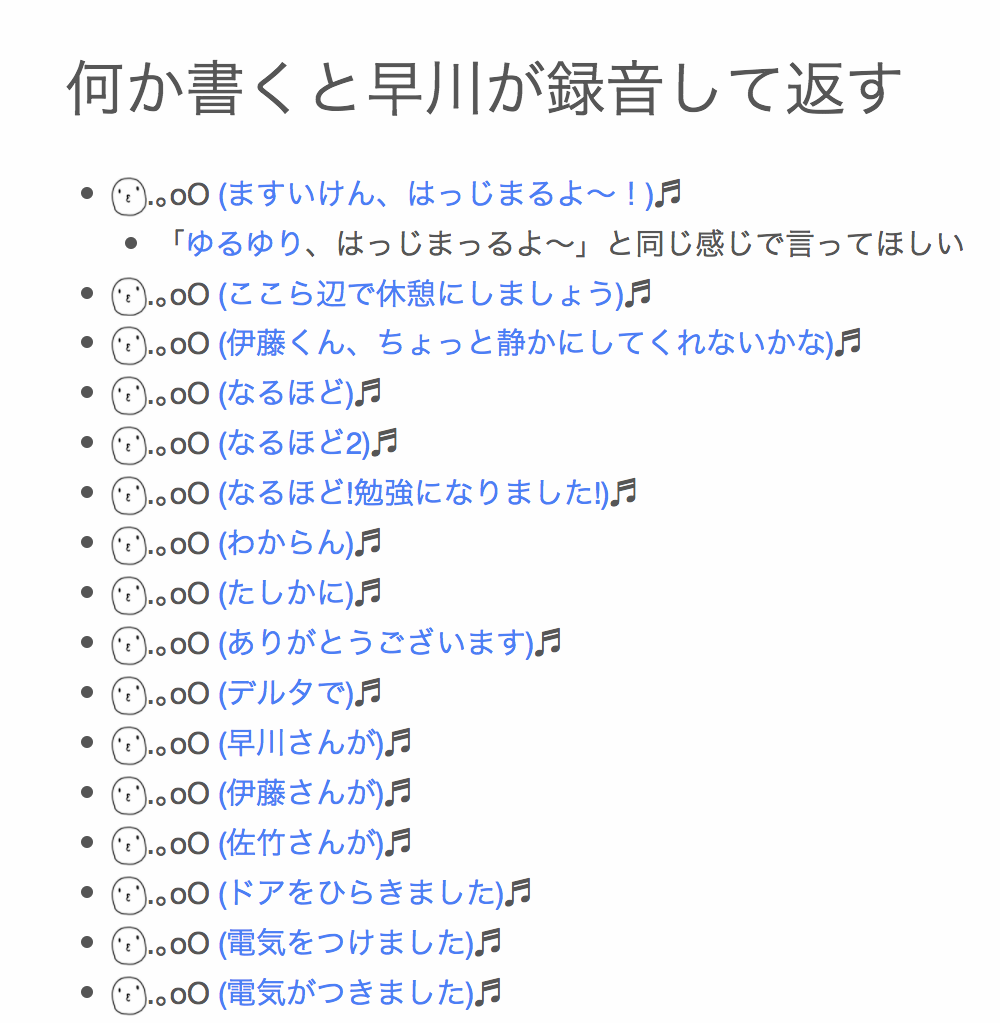
\includegraphics[width=9cm]{images/hayakawa.png}}
\caption{音声素材ページ}
\label{hayakawa}
\end{figure}

\subsubsection{単語帳を作る}
発音が難しい英単語等をまとめ、その音声を埋め込んだ図\ref{word}のような単語帳が作られた。
マウスカーソルを単語に重ねるだけで発音を確認できるので、より印象に残るものとなった。

\begin{figure}[H]
\centering
\fbox{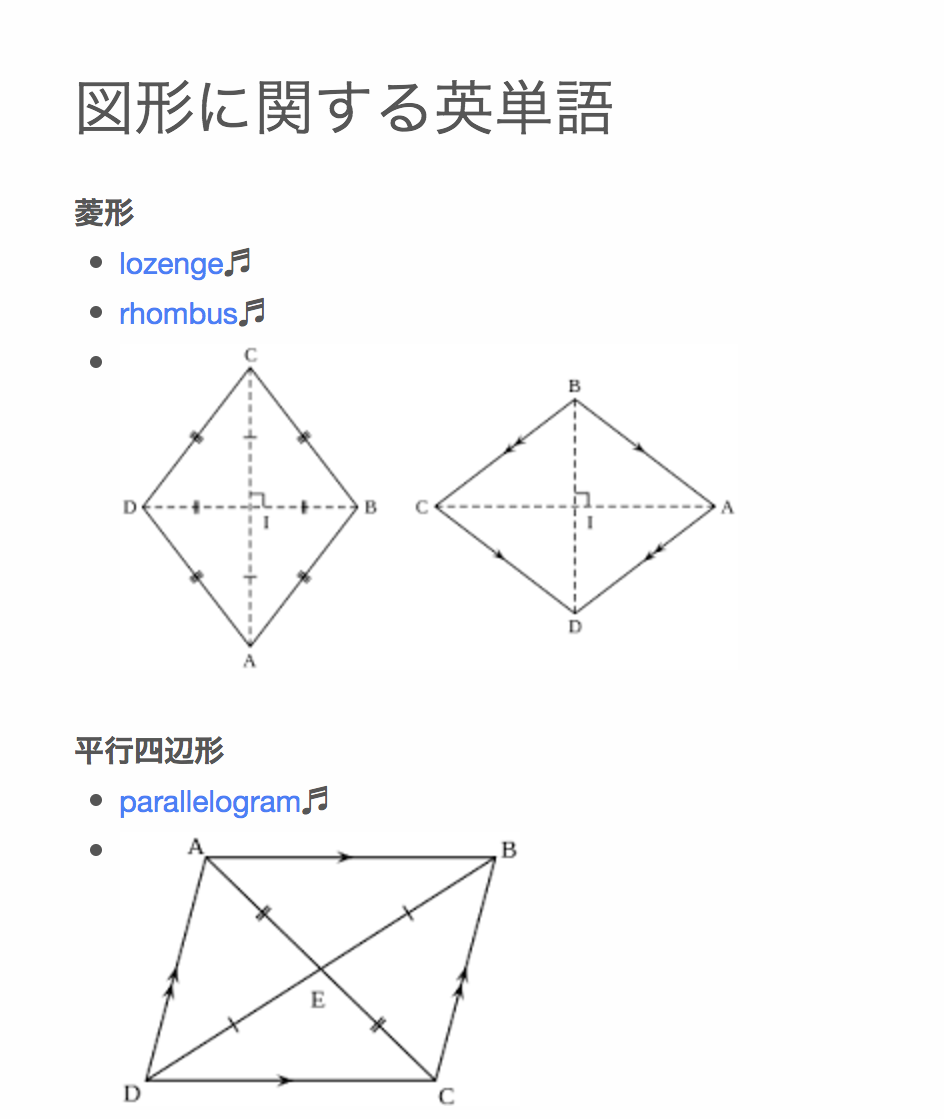
\includegraphics[width=9cm]{images/word.png}}
\caption{音声つき単語帳}
\label{word}
\end{figure}

\section{プライバシー問題}
簡単に録音できるため他者に対するプライバシー侵害の可能性があり、
社会で導入されることに対する心理的障壁は非常に高いと考えられる\cite{Kawamura}。

また、録音された音声に対してユーザ認証を行っていないため、
実際に公開して運用する場合は、ユーザのプライバシーに配慮した様々な対策が必要である。